\begin{comment}
\documentclass[10pt]{article}
\usepackage{fullpage, graphicx, url}
\setlength{\parskip}{1ex}
\setlength{\parindent}{0ex}
\title{nestedap}
\begin{document}


\begin{tabular}{ccc}
The Alternative Csound Reference Manual & & \\
Previous & &Next

\end{tabular}

%\hline 
\end{comment}
\section{nestedap}
nestedap�--� Three different nested all-pass filters. \subsection*{Description}


  Three different nested all-pass filters, useful for implementing reverbs. 
\subsection*{Syntax}


 ar \textbf{nestedap}
 asig, imode, imaxdel, idel1, igain1 [, idel2] [, igain2] [, idel3] [, igain3] [, istor]
\subsection*{Initialization}


 \emph{imode}
 -- operating mode of the filter: 


 
\begin{itemize}
\item 

 1 = simple all-pass filter

\item 

 2 = single nested all-pass filter

\item 

 3 = double nested all-pass filter


\end{itemize}


 \emph{idel1}
, \emph{idel2}
, \emph{idel3}
 -- delay times of the filter stages. Delay times are in seconds and must be greater than zero. \emph{idel1}
 must be greater than the sum of \emph{idel2}
 and \emph{idel3}
. 


 \emph{igain1}
, \emph{igain2}
, \emph{igain3}
 -- gain of the filter stages. 


 \emph{imaxdel}
 -- will be necessary if k-rate delays are implemented. Not currently used. 


 \emph{istor}
 -- Skip initialization if non-zero (default: 0). 
\subsection*{Performance}


 \emph{asig}
 -- input signal 


  If \emph{imode}
 = 1, the filter takes the form: 


 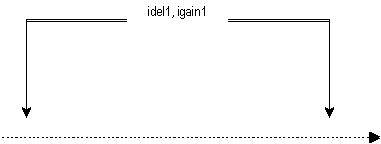
\includegraphics[scale=1]{imode1} 


 Picture of imode 1 filter.


  If \emph{imode}
 = 2, the filter takes the form: 


 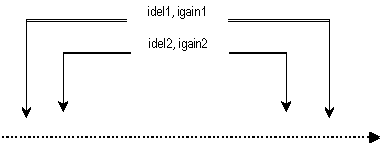
\includegraphics[scale=1]{imode2} 


 Picture of imode 2 filter.


  If \emph{imode}
 = 3, the filter takes the form: 


 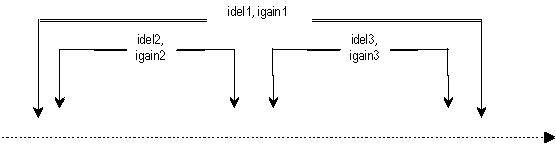
\includegraphics[scale=1]{imode3} 


 Picture of imode 3 filter.
\subsection*{Examples}


  Here is an example of the nestedap opcode. It uses the files \emph{nestedap.orc}
, \emph{nestedap.sco}
, and \emph{beats.wav}
. 


 \textbf{Example 1. Example of the nestedap opcode.}

\begin{lstlisting}
/* nestedap.orc */
sr = 44100
kr = 4410
ksmps = 10
nchnls = 2

instr 5
  insnd     =           p4
  gasig     diskin insnd, 1
endin

instr 10
  imax      =           1
  idel1     =           p4/1000
  igain1    =           p5
  idel2     =           p6/1000
  igain2    =           p7
  idel3     =           p8/1000
  igain3    =           p9
  idel4     =           p10/1000
  igain4    =           p11
  idel5     =           p12/1000
  igain5    =           p13
  idel6     =           p14/1000
  igain6    =           p15

  afdbk     init 0

  aout1     nestedap gasig+afdbk*.4, 3, imax, idel1, igain1, idel2, igain2, idel3, igain3
  
  aout2     nestedap aout1, 2, imax, idel4, igain4, idel5, igain5

  aout      nestedap aout2, 1, imax, idel6, igain6

  afdbk     butterlp aout, 1000

            outs gasig+(aout+aout1)/2, gasig-(aout+aout1)/2
  
gasig     =           0
endin
/* nestedap.orc */
        
\end{lstlisting}
\begin{lstlisting}
/* nestedap.sco */
f1 0 8192 10 1

; Diskin
;   Sta  Dur  Soundin
i5  0    3    "beats.wav"

; Reverb
;   St  Dur  Del1 Gn1  Del2  Gn2  Del3  Gn3  Del4  Gn4  Del5  Gn5  Del6  Gn6
i10 0   4    97   .11  23   .07   43   .09   72    .2   53    .2   119   .3
e
/* nestedap.sco */
        
\end{lstlisting}
\subsection*{Credits}


 


 


\begin{tabular}{cc}
Author: Hans Mikelson &February 1999

\end{tabular}



 


 New in Csound version 3.53


 The example was updated May 2002, thanks to Hans Mikelson
%\hline 


\begin{comment}
\begin{tabular}{lcr}
Previous &Home &Next \\
nchnls &Up &nlfilt

\end{tabular}


\end{document}
\end{comment}
